\documentclass[../dissertation.tex]{subfiles}

\begin{document}

\subsection{Experiment 3 - CPU Clock Speed}
\label{experiment3-cpu-speed}

The purpose of this experiment was to identify whether the limited CPU power of the Raspberry Pi system was playing a significant role in the bottlenecking of message communication at higher frequencies.

This is achieved by underclocking the Raspberry Pi 3 Model B CPU by 25\%, and 50\%. The reason to do this instead of changing the hardware (for example changing to desktop machines) is that this method keeps variables such as CPU architecture, disk speed, and software stack the same across the experiment.

The hypothesis for the experiment was that frequencies which we had previously seen high message latency for would result in even higher latency, and the maximum `low latency' frequency would be lower as the core clock speed reduces.

One potential issue is that modern CPUs often underclock (reduce the clock speed and voltage) themselves, thus it can be hard to know exactly what CPU speed is being used throughout the experiment. Thus, several times throughout the experiment the current CPU speed was checked, and verified to be running at the specified maximum frequency.

\subsubsection{Results}

The results agreed with the hypothesis. At 100\% CPU clock speed, only the highest 3 frequencies demonstrated sustained degradation of performance, however at 75\% the top 5 frequencies showed, and at 50\% the top 7 had reduced performance.

\begin{figure}[H]
\centering
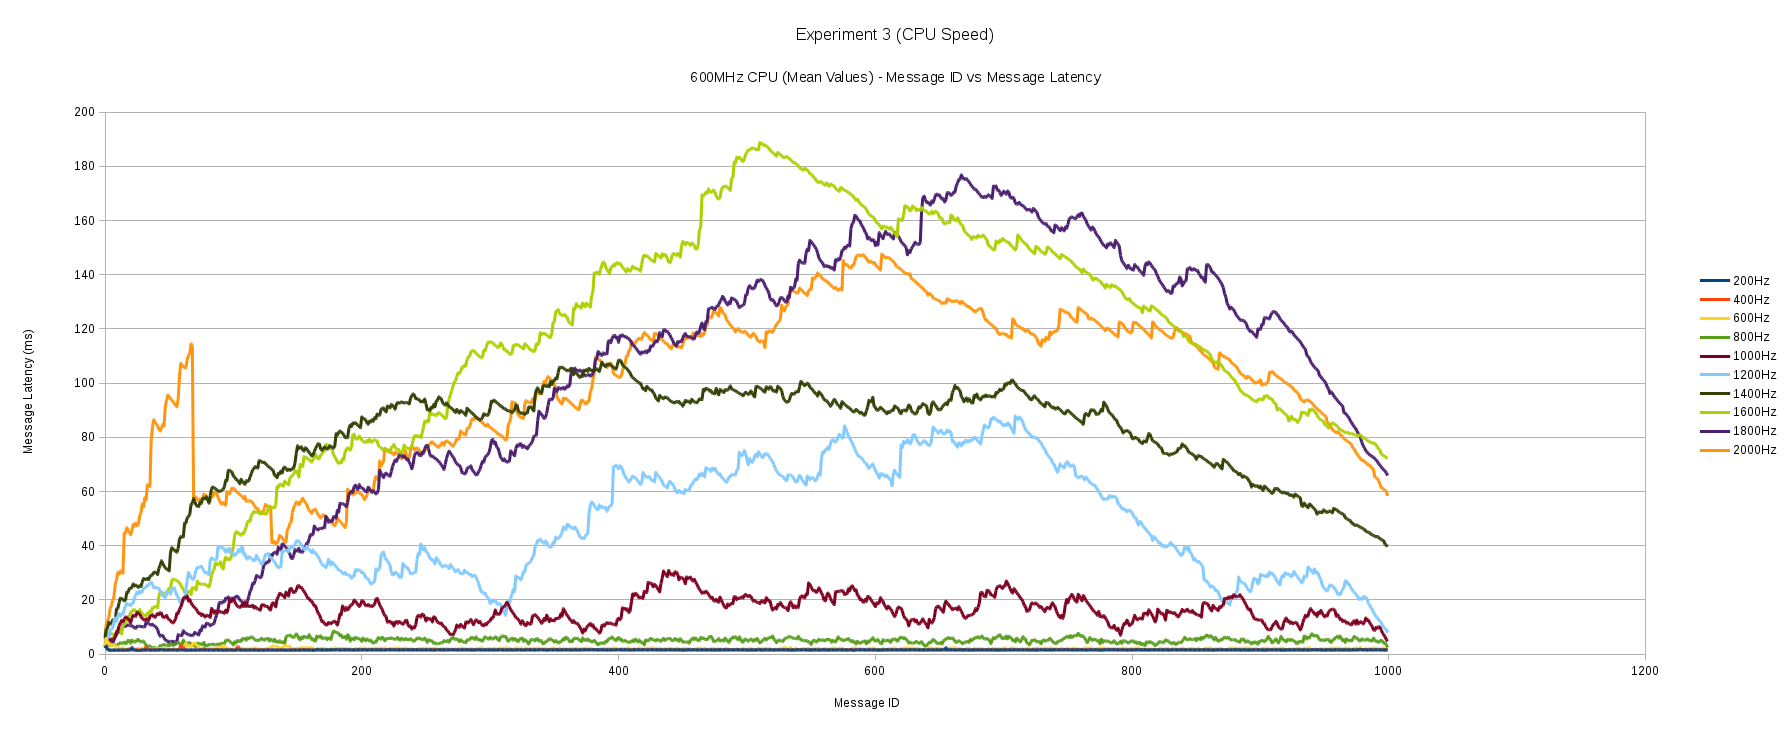
\includegraphics[width=\textwidth]{images/experiment3/50_clockspeed_mean_values_by_freq_pretty.png}
\caption{Experiment 3 - 100\% CPU Speed, All Frequencies}
\label{exp3-cpu100}
\end{figure}

Overall message latency was also increased as CPU core clock speed reduced. Even at the lowest frequency of 200Hz, 100\% CPU had an average message latency of 1.188ms, 75\%'s was 1.399, and 50\%'s was 1.609ms. Higher message frequencies demonstrated greater differences as shown in Figure \ref{exp3-averages}.

\begin{figure}[H]
\centering
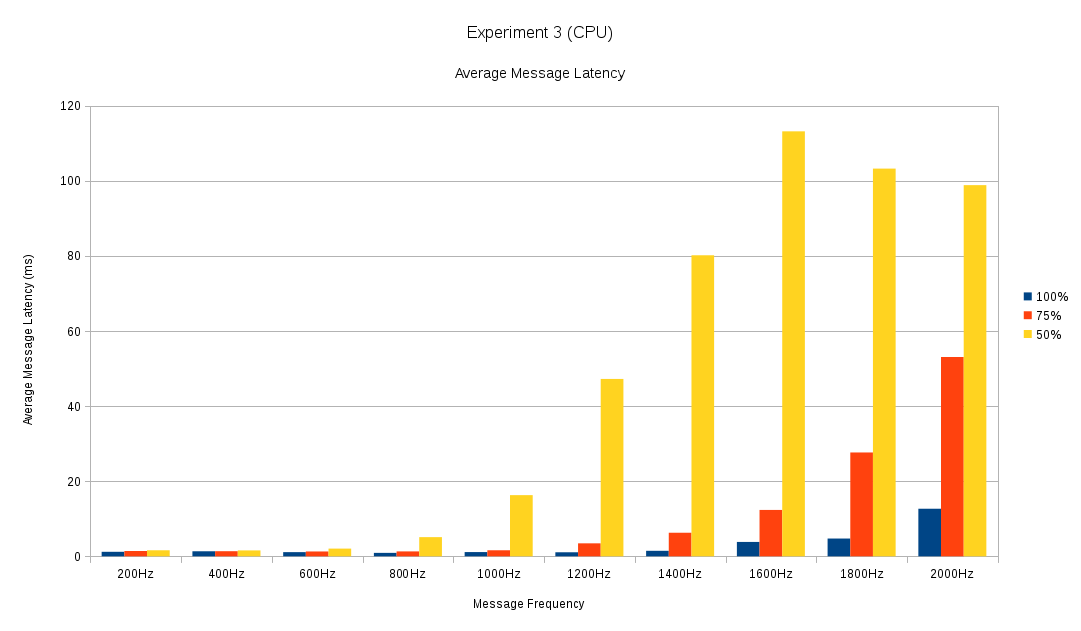
\includegraphics[width=\textwidth]{images/experiment3/average_per_frequency_graph.png}
\caption{Experiment 3 - All CPU Speeds, All Frequencies}
\label{exp3-averages}
\end{figure}

\textit{We can conclude from these results that the CPU performance of the host machines can be a limiting factor for high frequency ROS communication, and thus CPU utilisation is an important metric when evaluating why a ROS system is experiencing poor performance.}

\end{document}
